% !TEX program = xelatex
\documentclass[UTF8,fontset=fandol,a4paper,12pt]{ctexart}

\usepackage[left=24mm,right=24mm,top=24mm,bottom=24mm]{geometry}
\usepackage{graphicx}
\usepackage{booktabs}
\usepackage{tabularx}
\usepackage{array}
\usepackage{longtable}
\usepackage{float}
\usepackage{caption}
\usepackage{xcolor}
\usepackage{hyperref}
\usepackage{fancyhdr}
\usepackage{enumitem}
\usepackage{listings}
\usepackage{setspace}
\usepackage{titlesec}

\definecolor{QYYNavy}{HTML}{183654}
\definecolor{QYYTeal}{HTML}{007C91}
\definecolor{QYYLight}{HTML}{EEF4F7}
\definecolor{QYYGold}{HTML}{D99A24}
\definecolor{QYYGray}{HTML}{5B6770}

\hypersetup{
  colorlinks=true,
  linkcolor=QYYTeal,
  urlcolor=QYYTeal,
  citecolor=QYYTeal,
  pdftitle={机器人集成小组项目1实验报告},
  pdfauthor={QYY},
  pdfsubject={YOLOv8, Jetson Orin NX, ROS2}
}

\pagestyle{fancy}
\setlength{\headheight}{15pt}
\fancyhf{}
\fancyhead[L]{\small\color{QYYGray}机器人集成小组项目1}
\fancyhead[R]{\small\color{QYYGray}YOLOv8 / Jetson / ROS2}
\fancyfoot[C]{\small\color{QYYGray}\thepage}
\renewcommand{\headrulewidth}{0.4pt}

\titleformat{\section}
  {\Large\bfseries\color{QYYNavy}}
  {\thesection.}{0.6em}{}
\titleformat{\subsection}
  {\large\bfseries\color{QYYTeal}}
  {\thesubsection}{0.6em}{}

\setlist[itemize]{leftmargin=2em,itemsep=0.2em,topsep=0.3em}
\setstretch{1.28}
\captionsetup{font=small,labelfont=bf,textfont=it}
\graphicspath{{figures/}}

\lstset{
  basicstyle=\ttfamily\small,
  backgroundcolor=\color{QYYLight},
  frame=single,
  rulecolor=\color{QYYTeal},
  breaklines=true,
  columns=fullflexible,
  showstringspaces=false,
  xleftmargin=0.5em,
  xrightmargin=0.5em
}

\newcommand{\metric}[2]{%
  \begin{minipage}[t]{0.47\textwidth}
    \colorbox{QYYLight}{\parbox{0.92\linewidth}{%
      \centering\color{QYYNavy}\bfseries #1\\[2pt]
      \Large\color{QYYTeal}#2}}
  \end{minipage}}

\begin{document}

\begin{titlepage}
  \thispagestyle{empty}
  \vspace*{18mm}
  \begin{center}{\color{QYYTeal}\rule{0.95\textwidth}{2.2pt}}\end{center}
  \vspace{12mm}
  \begin{center}
    {\Huge\bfseries\color{QYYNavy}机器人集成小组项目1实验报告\par}
    \vspace{8mm}
    {\LARGE\color{QYYTeal}基于 YOLOv8 和 Jetson Orin NX 的\par}
    \vspace{3mm}
    {\LARGE\color{QYYTeal}桌面目标检测与 ROS2 发布\par}
  \end{center}
  \vspace{10mm}

  \begin{center}
    \metric{数据集}{1000 张图片}\hfill
    \metric{正式测试}{21/22，95.45\%}\\[7mm]
    \metric{完整循环速度}{平均 16.77 FPS}\hfill
    \metric{推理阈值}{conf = 0.70}
  \end{center}

  \vfill
  \renewcommand{\arraystretch}{1.5}
  \noindent\begin{tabularx}{\textwidth}{>{\bfseries\color{QYYNavy}}l X}
    提交人 & QYY \\
    项目仓库 & \url{https://github.com/ccx8kg5qpd-debug/robotics-group-project-1} \\
    报告模板 & 个人设计 LaTeX 模板 \\
    报告日期 & 2026-08-29 \\
  \end{tabularx}
  \vspace{10mm}
  \begin{center}{\color{QYYTeal}\rule{0.95\textwidth}{2.2pt}}\end{center}
\end{titlepage}

\tableofcontents
\newpage

\section{实验名称}

机器人集成小组项目1：基于 YOLOv8 和 Jetson Orin NX 的桌面目标检测与 ROS2 发布。

\section{实验目的}

本实验面向桌面场景中的 bottle 和 mouse 两类物体，完成数据整理与标注、YOLO 目标检测模型训练、Jetson Orin NX GPU 部署、实时检测结果显示及 ROS2 发布。实时界面需要显示 bounding box、class、confidence 和完整循环 FPS；正式测试不少于 20 个实例，正确识别率不低于 80\%，Jetson 实际运行速度不低于 5 FPS。

\section{实验设备与软件环境}

\subsection{训练环境}

\begin{itemize}
  \item Mac，使用 Apple MPS 训练；
  \item YOLOv8n，输入尺寸 640，训练 100 epochs；
  \item 训练产物记录的 Ultralytics 版本为 8.4.128。
\end{itemize}

\subsection{部署环境}

\begin{table}[H]
\centering
\caption{Jetson 部署环境}
\begin{tabularx}{0.9\textwidth}{>{\bfseries}l X}
\toprule
项目 & 配置 \\
\midrule
硬件 & NVIDIA Jetson Orin NX，USB 摄像头 \\
操作系统 & Ubuntu 22.04.5 LTS \\
JetPack / L4T & JetPack 6.2.1 / L4T R36.4.4 \\
Python & 3.10.12 \\
ROS2 & Humble \\
CUDA & 约 12.6 \\
Ultralytics & Jetson 部署记录为 8.4.132 \\
PyTorch & 与 JetPack 6 / CUDA 12.6 匹配的 ARM64 版本 \\
\bottomrule
\end{tabularx}
\end{table}

部署过程验证了 \texttt{ROS2 OK}、\texttt{YOLO OK} 以及 \texttt{torch.cuda.is\_available() == True}。摄像头由 \texttt{cv2.VideoCapture(0)} 打开。

\section{数据集构建}

\subsection{自采数据}

项目最初使用 iPhone 拍摄 30 张真实桌面图片，包括 bottle、mouse 和两类同时出现的场景。原始格式主要为 HEIC，之后转换为 JPEG。早期曾使用 YOLOv8x COCO 预训练模型辅助检查自采图片中的目标框，并人工查看预览结果。该过程只服务于早期自采数据整理。

\subsection{外部公开数据}

为扩充训练规模，加入 970 张 COCO 2017 图片。外部标注直接来自 COCO 官方 instance annotations，经类别映射后转换为 YOLO 格式，并非由早期自动标注程序生成。外部图片仅用于课程教学和科研实验，每张图片的来源 URL、许可名称、许可 URL、COCO ID 与 SHA-256 均保存在 \texttt{dataset/source\_info/source\_manifest.csv}。

\subsection{最终划分与类别统计}

\begin{table}[H]
\centering
\caption{最终数据划分}
\begin{tabular}{lrrrrrr}
\toprule
划分 & 图片/标注 & 自采 & 外部 & bottle 框 & mouse 框 \\
\midrule
train & 800 & 20 & 780 & 2358 & 696 \\
val   & 100 & 5  & 95  & 227  & 82  \\
test  & 100 & 5  & 95  & 297  & 95  \\
\midrule
合计  & 1000 & 30 & 970 & 2882 & 873 \\
\bottomrule
\end{tabular}
\end{table}

类别映射为 \texttt{0=bottle}、\texttt{1=mouse}。标注采用 YOLO 归一化格式：\texttt{class x\_center y\_center width height}。

\section{数据质量检查}

数据质量检查遍历 1000 张图片和 1000 个标注文件，检查图片/标注文件名对应、空标注、类别 ID、字段数量、坐标解析、归一化范围、正宽高、边框越界、图片完整性以及跨划分 SHA-256 完全重复。

核验结果为：缺标注 0、孤立标注 0、空标注 0、非法类别 0、非法或越界坐标 0、损坏图片 0、跨划分完全重复图片 0。实际总框数为 bottle 2882、mouse 873。历史统计中的 bottle 2855、mouse 846 是仅针对 970 张外部数据的统计，不能替代最终 1000 张数据的真实数量。

\section{模型训练}

训练命令如下：

\begin{lstlisting}
yolo detect train \
  model=yolov8n.pt \
  data=final_dataset/data.yaml \
  epochs=100 \
  imgsz=640 \
  device=mps
\end{lstlisting}

训练完成 100 epochs，\texttt{results.csv} 最后一行记录累计时间 14421.7 秒，约 4.006 小时。最终部署模型使用 \texttt{weights/best.pt}，大小 6,244,266 bytes。

\begin{figure}[H]
  \centering
  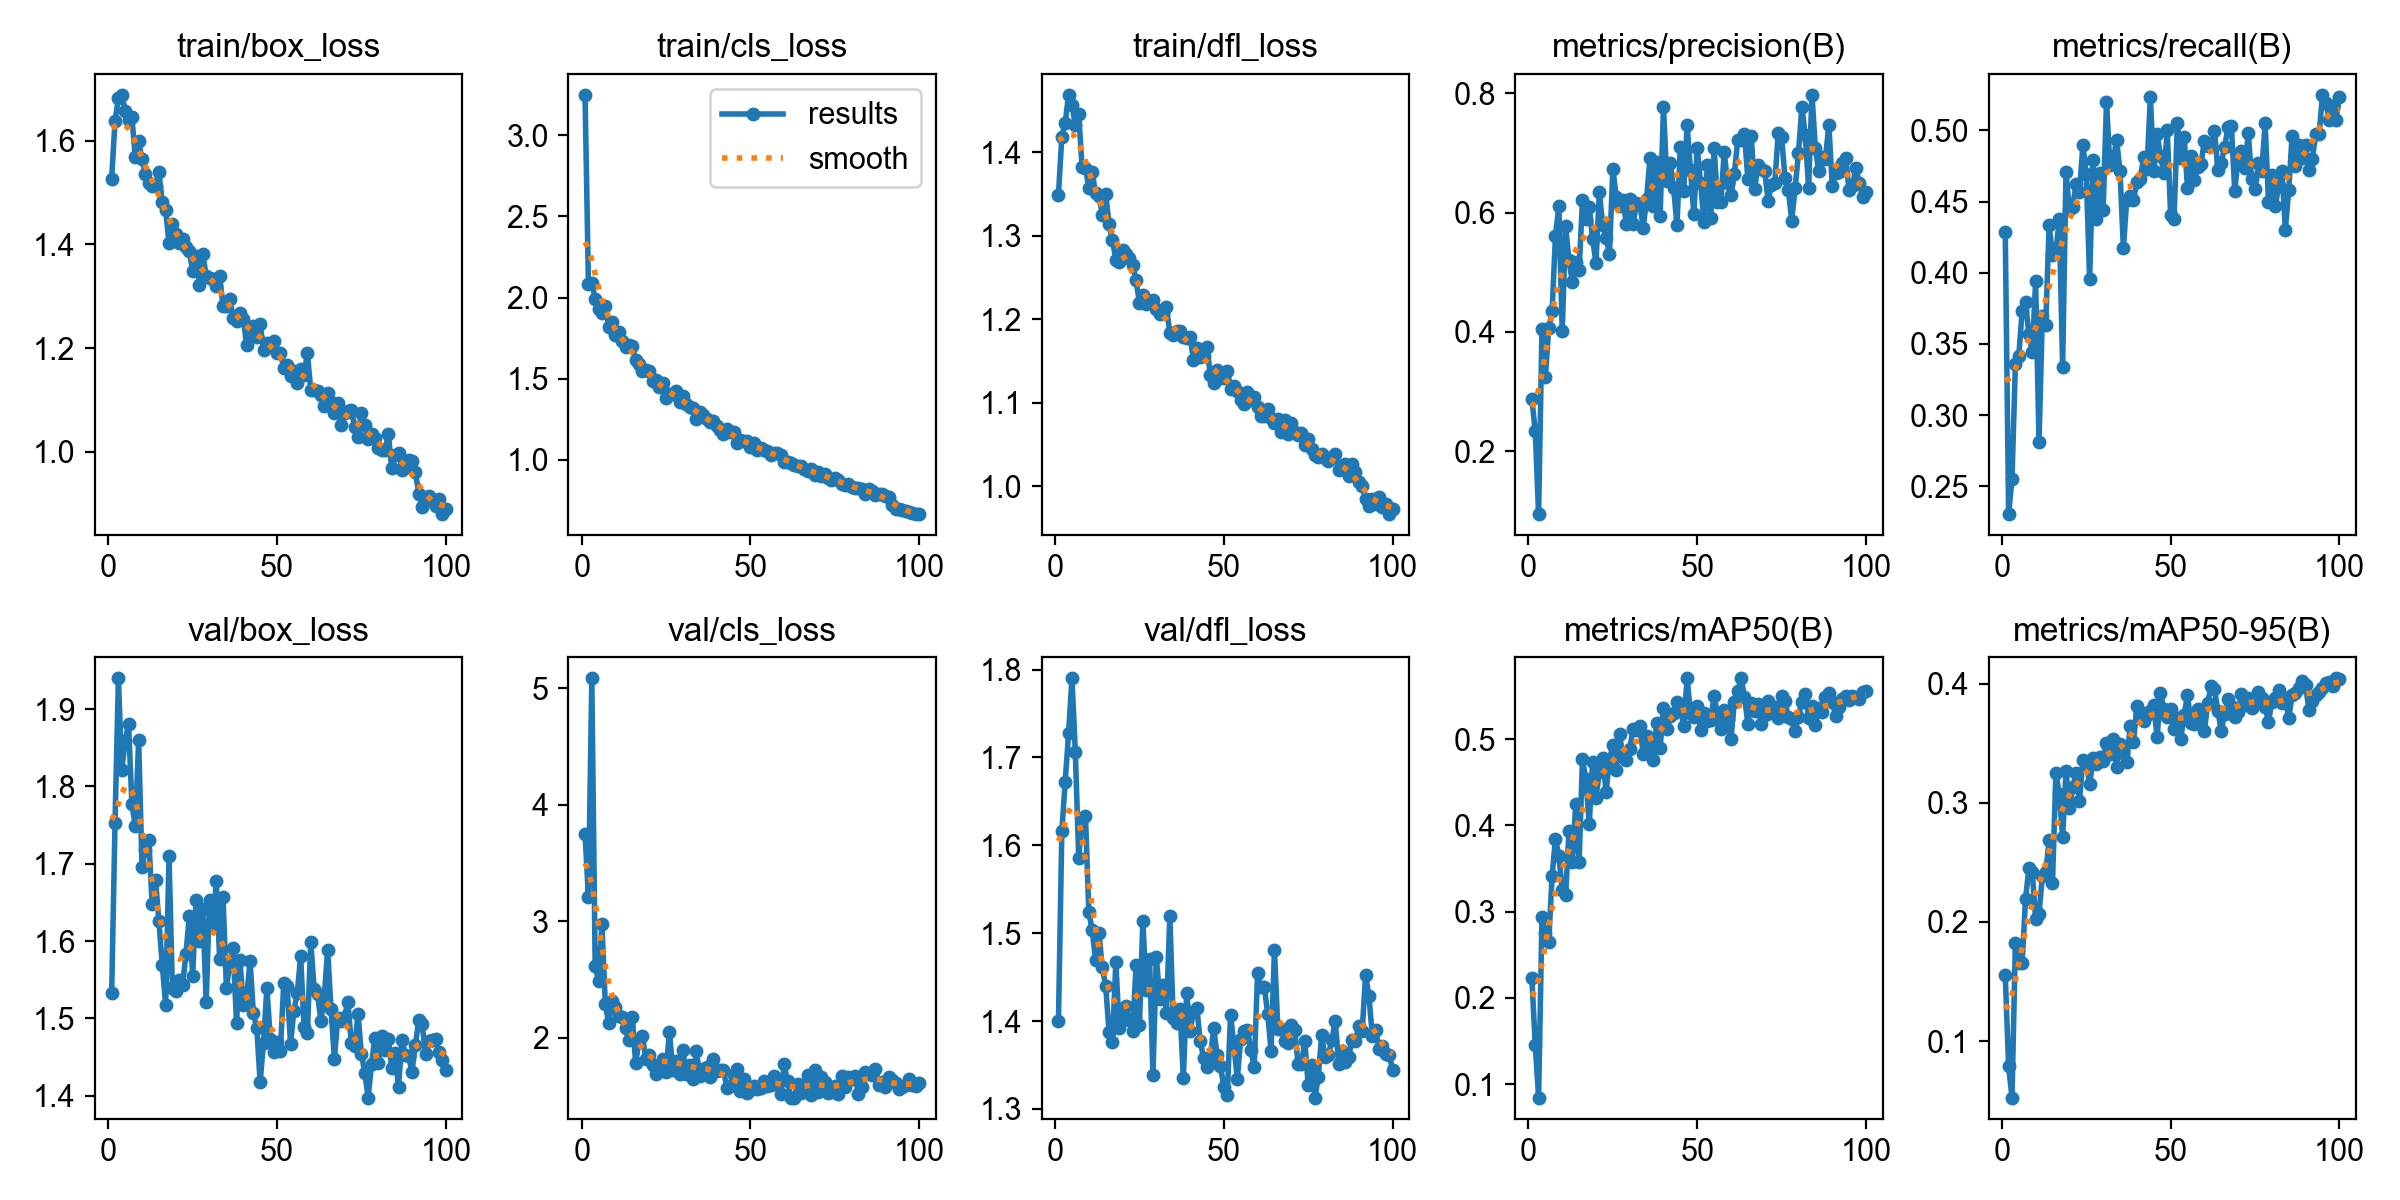
\includegraphics[width=0.95\textwidth]{training_results.png}
  \caption{YOLOv8n 训练曲线}
\end{figure}

\section{模型评估}

训练记录中 mAP50-95 最高的第 99 epoch 与第 100 epoch 汇总指标如下。

\begin{table}[H]
\centering
\caption{训练记录汇总指标}
\begin{tabular}{lrrrr}
\toprule
来源 & P & R & mAP50 & mAP50-95 \\
\midrule
第 99 epoch  & 0.625 & 0.508 & 0.554 & 0.404 \\
第 100 epoch & 0.634 & 0.523 & 0.556 & 0.404 \\
\bottomrule
\end{tabular}
\end{table}

使用保存的 \texttt{best.pt} 在 Mac CPU、Ultralytics 8.4.128 上对 100 张 val 图片重新评估，得到：

\begin{table}[H]
\centering
\caption{best.pt 复评结果}
\begin{tabular}{lrrrrrr}
\toprule
类别 & images & instances & P & R & mAP50 & mAP50-95 \\
\midrule
all    & 100 & 309 & 0.676 & 0.488 & 0.555 & 0.405 \\
bottle & 63  & 227 & 0.592 & 0.379 & 0.418 & 0.276 \\
mouse  & 62  & 82  & 0.760 & 0.598 & 0.691 & 0.533 \\
\bottomrule
\end{tabular}
\end{table}

\begin{figure}[H]
  \centering
  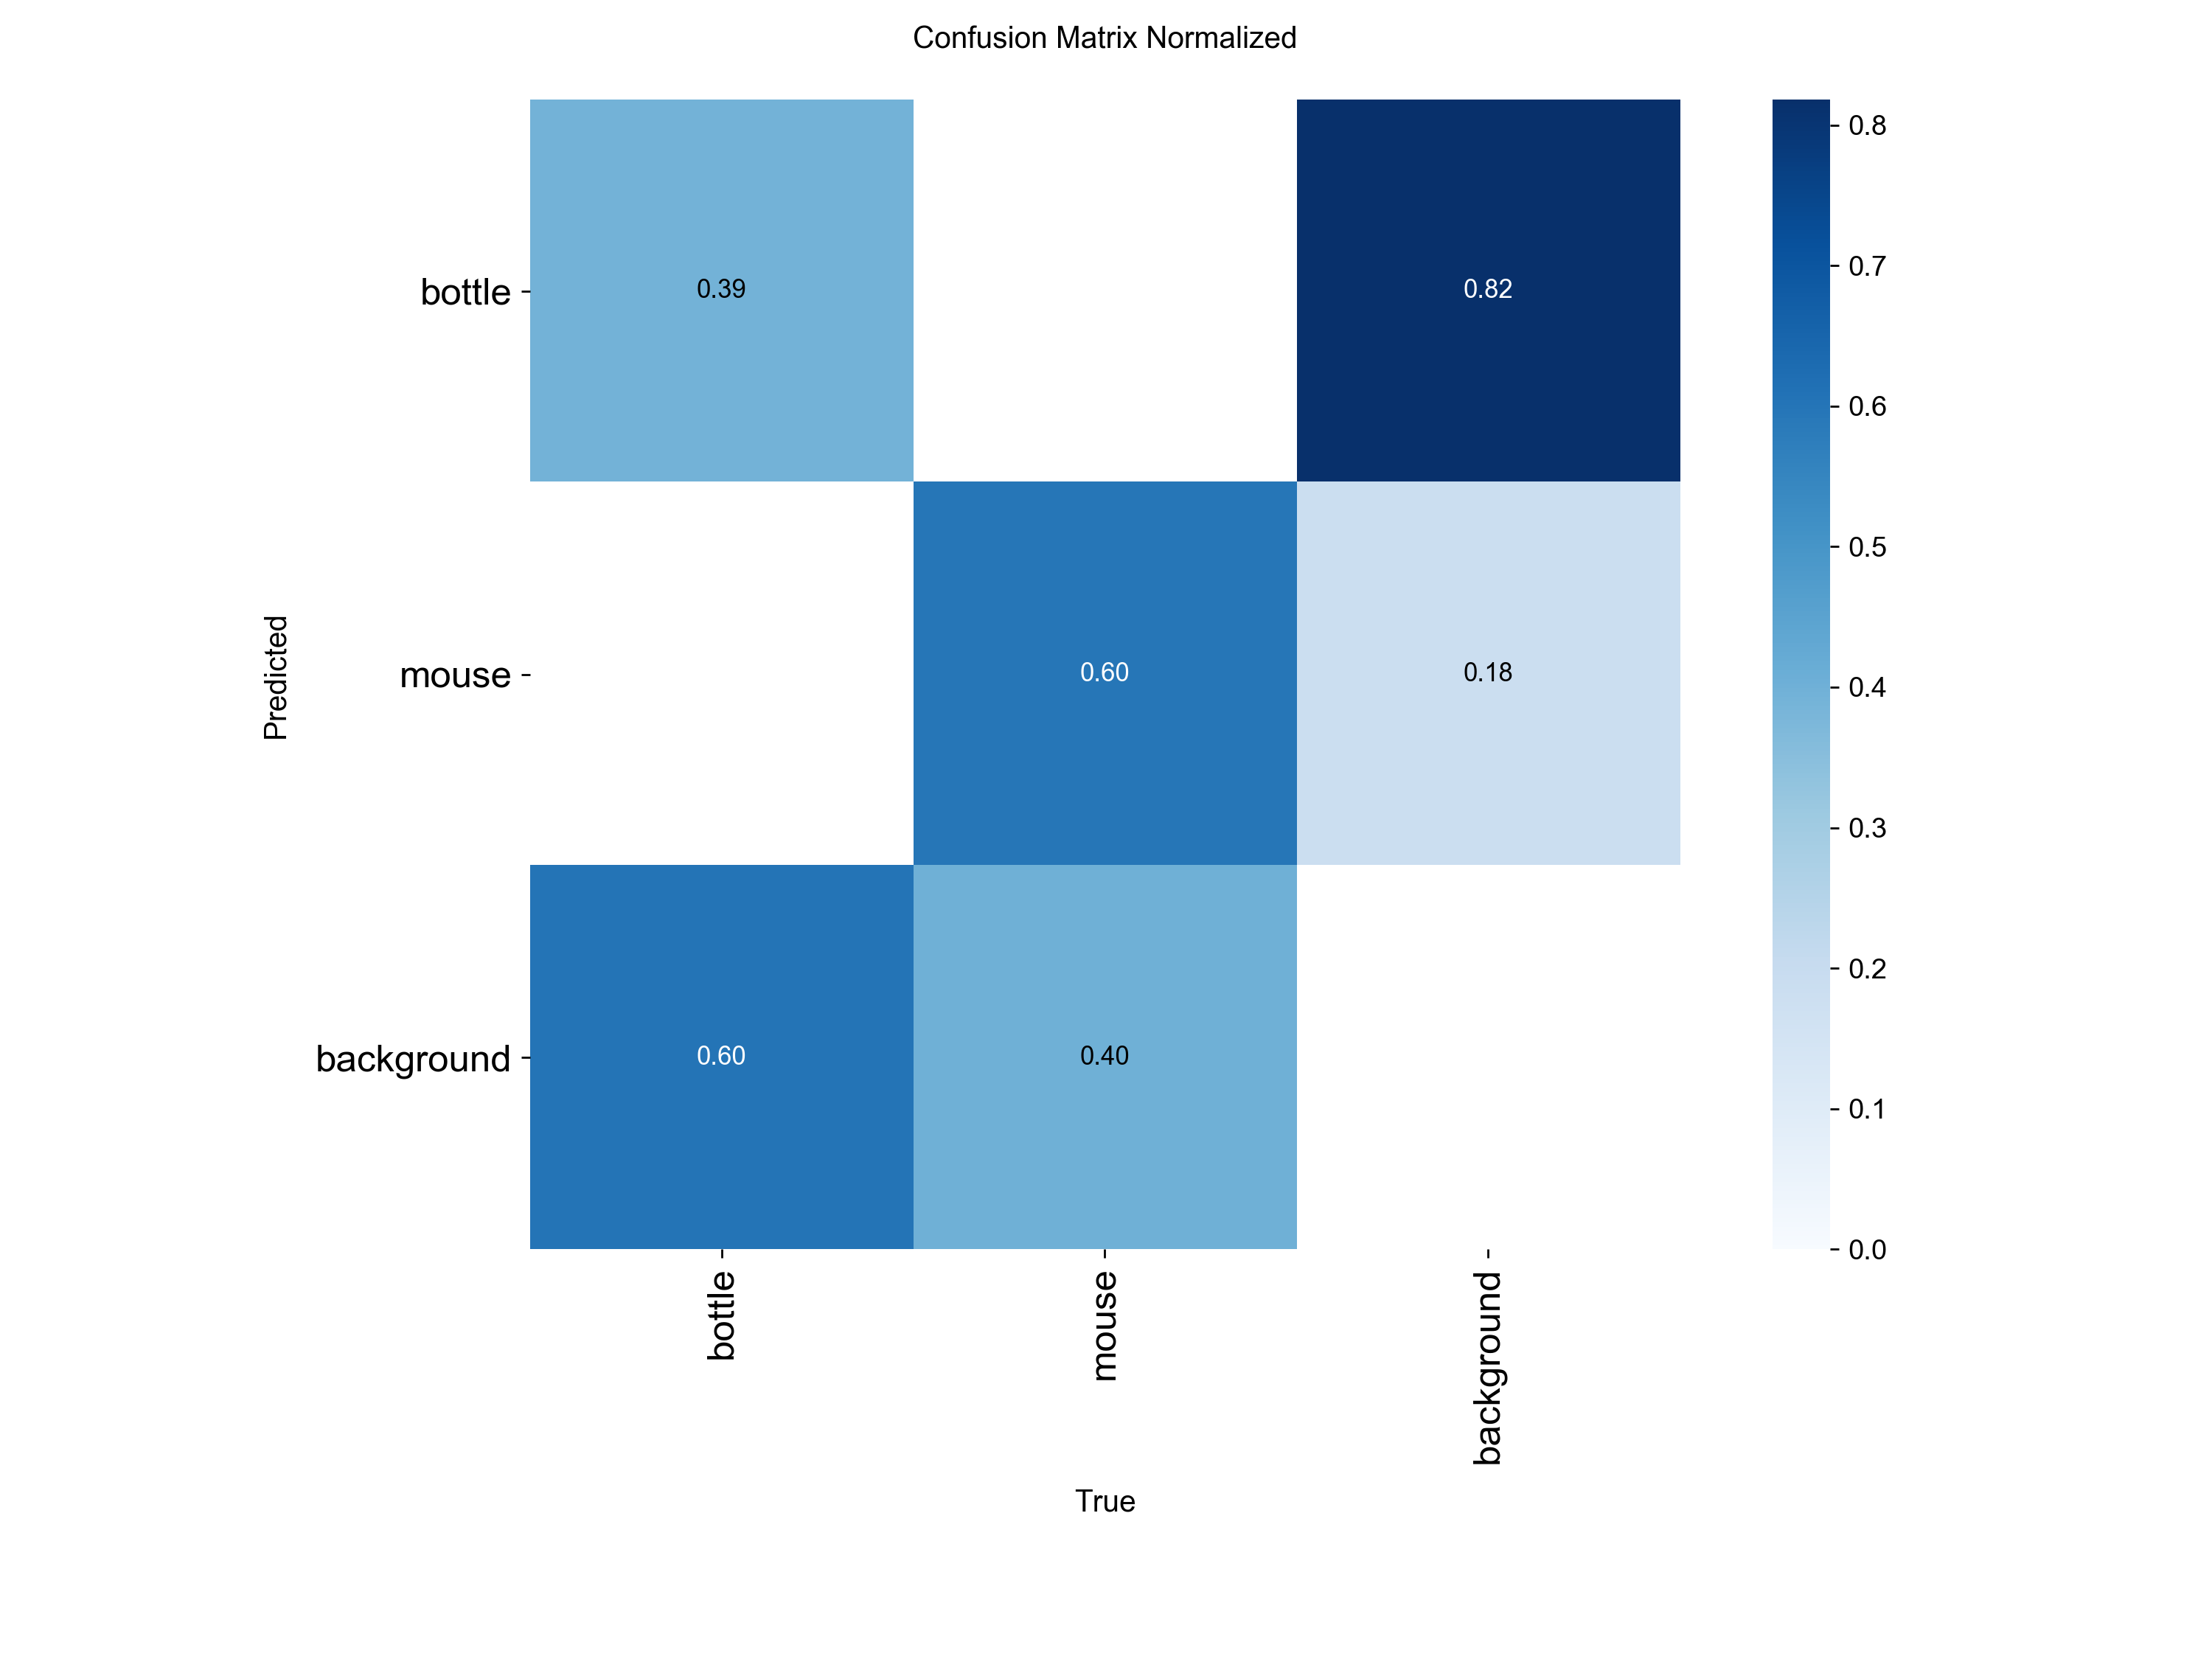
\includegraphics[width=0.62\textwidth]{confusion_matrix_normalized.png}
  \caption{归一化混淆矩阵}
\end{figure}

\section{Jetson 部署与实时程序}

最终权重部署于 \texttt{/home/nvidia/qyy\_object\_detection}。为保证 GPU 可用，安装与 JetPack 6 / CUDA 12.6 匹配的 ARM64 PyTorch，并处理 \texttt{libcudss.so.0} 动态库依赖，将 \texttt{/usr/lib/aarch64-linux-gnu/libcudss/12} 加入 \texttt{LD\_LIBRARY\_PATH}。

\texttt{detect\_realtime.py} 和 \texttt{ros2\_detect.py} 均加载当前目录下的 \texttt{best.pt}，使用 camera 0、\texttt{device=0} 和 \texttt{conf=0.70}。程序显示 bbox、class 与 confidence，并用最近 30 帧完整循环耗时计算平滑 FPS。按 \texttt{s} 保存正确案例、按 \texttt{e} 保存错误案例、按 \texttt{q} 退出。

\section{ROS2 集成}

\texttt{ros2\_detect.py} 定义 ROS2 node \texttt{qyy\_yolo\_detector}，创建 \texttt{/qyy/detections} publisher，消息类型为 \texttt{std\_msgs/msg/String}。每帧发布 JSON 字符串，包含 FPS、类别、置信度与 bbox。

\begin{lstlisting}
{
  "fps": 18.2,
  "detections": [
    {
      "class": "bottle",
      "confidence": 0.93,
      "bbox": [100, 100, 300, 400]
    }
  ]
}
\end{lstlisting}

上述数字仅用于说明消息格式，不是实验测试结果。项目使用 \texttt{ros2 topic list} 与 \texttt{ros2 topic echo /qyy/detections} 验证 topic 能持续输出实时 JSON 检测结果。

\section{正式测试与 FPS}

\texttt{correct\_cases} 和 \texttt{error\_cases} 中的保存帧作为正式测试实例。共记录 22 个实例，其中 21 个正确、1 个错误，正确率为 95.45\%，高于作业要求的 80\%。唯一错误是横放 bottle 漏检；同一帧中的 mouse 以 0.96 置信度正确识别，没有发生错误类别。

\begin{table}[H]
\centering
\caption{正式测试汇总}
\begin{tabular}{rrrrrl}
\toprule
测试实例 & 正确 & 错误 & 正确率 & 作业要求 & 结论 \\
\midrule
22 & 21 & 1 & 95.45\% & $\geq$20 且 $\geq$80\% & 达标 \\
\bottomrule
\end{tabular}
\end{table}

22 张保存帧显示的完整循环 FPS 为 16.6-16.9，算术平均约 16.77 FPS，最低值、最高值和平均值均高于 5 FPS。该数值包含摄像头采集、推理、绘制与显示，不是由单独 inference time 反算。

\begin{figure}[H]
  \centering
  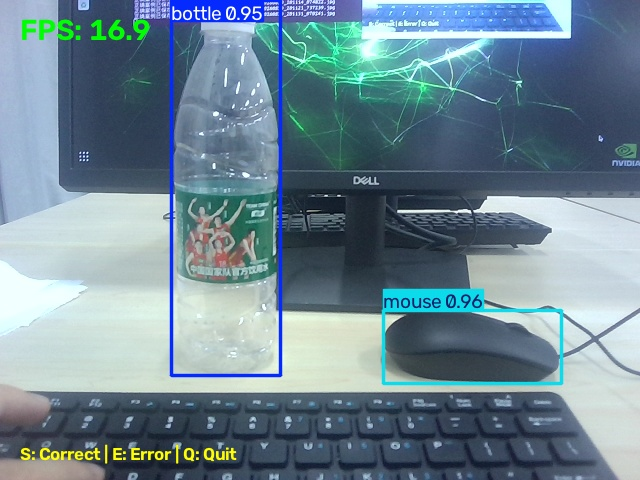
\includegraphics[width=0.48\textwidth]{correct_case.jpg}
  \caption{bottle 与 mouse 双目标正确案例，FPS 16.9}
\end{figure}

\section{典型错误与改进}

\begin{figure}[H]
  \centering
  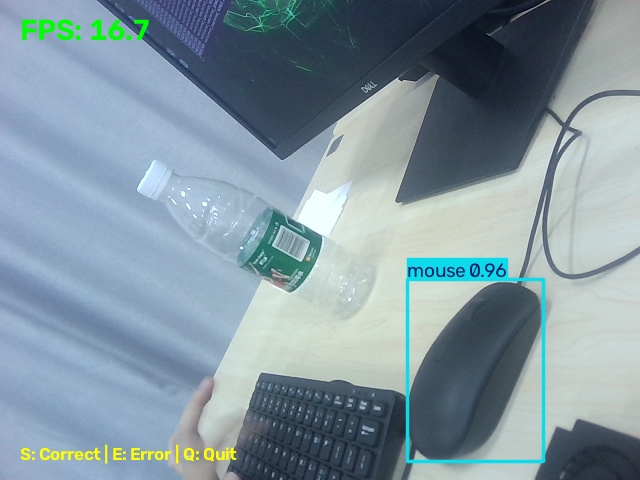
\includegraphics[width=0.48\textwidth]{error_case.jpg}
  \caption{真实错误案例：横放 bottle 漏检，mouse 正确识别}
\end{figure}

初期使用较低 confidence threshold 时，键盘区域曾被误识别为 mouse，出现过约 0.26 和约 0.63 的错误置信度。真实 mouse 常见约 0.96/0.98，真实 bottle 常见约 0.95/0.96。将推理阈值提高到 0.70 后，该类已知误检受到抑制。此处改动是推理阈值调整，并非重新训练模型。键盘误检图片未保留，因此只记录调试现象，不附模拟截图。

\section{演示视频}

最终演示视频原件为 \texttt{IMG\_9829.MOV}，原始画面 3840x2160、约 119.95 FPS、时长约 104.08 秒。课程提交包中包含 1920x1080、30 FPS、约 104.07 秒的 \texttt{final\_demo.mp4} 画面版。

分段抽帧确认视频展示了 Jetson 硬件、USB 摄像头、bottle、mouse、双目标检测、bbox/class/confidence/FPS 叠加，以及另一个终端持续输出 \texttt{/qyy/detections} JSON 消息。提交副本首帧和 100 秒位置均可正常解码。

\section{版本管理与个人仓库}

项目材料按数据说明、程序实现、实验结果和报告整理等内容阶段提交。个人仓库地址为：

\begin{center}
\url{https://github.com/ccx8kg5qpd-debug/robotics-group-project-1}
\end{center}

提交分为数据来源与说明、Jetson/ROS2 程序与模型、训练和正式测试结果、LaTeX 报告等阶段。图 \ref{fig:commits} 为报告编制时的真实本地 commit 记录；远程推送后可在上述 GitHub 仓库继续查看完整记录。

\begin{figure}[H]
  \centering
  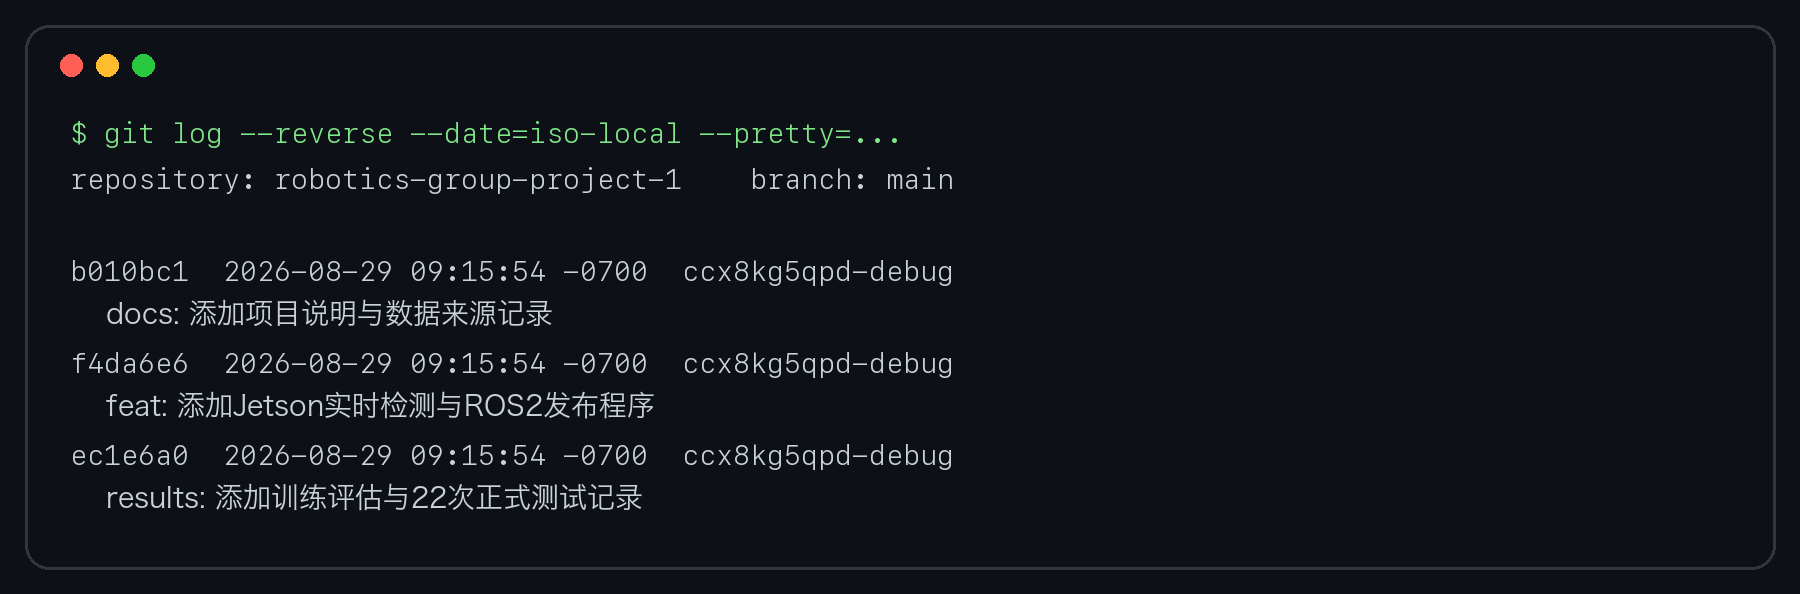
\includegraphics[width=\textwidth]{commit_history.png}
  \caption{Git 分阶段提交记录}
  \label{fig:commits}
\end{figure}

考虑到 GitHub 文件大小限制和外部图片许可，完整 1000 图数据集、原始演示视频及课程提交 ZIP 不在公共仓库重复发布。仓库保留 \texttt{data.yaml}、划分清单、数据质量报告和逐图来源/许可清单，完整材料随课程提交 ZIP 提交。

\section{实验问题与解决过程}

\begin{itemize}
  \item 数据来源表述：最终 1000 张中只有 30 张为自采，970 张来自 COCO 2017；
  \item Jetson PyTorch/CUDA 兼容：使用与 JetPack 6 / CUDA 12.6 匹配的 ARM64 PyTorch；
  \item 动态库问题：安装 \texttt{libcudss0-cuda-12} 并配置 \texttt{LD\_LIBRARY\_PATH}；
  \item 桌面误检：将推理置信度阈值调整为 0.70，抑制已知 keyboard-to-mouse 误检；
  \item ROS2 发布：采用 \texttt{std\_msgs/String} 发送 JSON，并通过 topic echo 验证。
\end{itemize}

\section{实验总结}

项目完成了 bottle 与 mouse 两类桌面目标的数据集整理、YOLOv8n 训练、Jetson Orin NX GPU 实时部署、bbox/class/confidence 显示、完整循环 FPS 测量、正确/错误案例保存及 ROS2 结果发布。数据集规模为 1000 张，best.pt 复评 mAP50-95 为 0.405。22 个正式测试实例中 21 个正确，正确率 95.45\%；平均完整循环速度约 16.77 FPS，满足测试数量、正确率和实时速度要求。最终演示视频、个人 Git 仓库、分阶段 commit 记录以及个人 LaTeX 报告模板均作为课程材料整理。

\end{document}
